\documentclass[twoside]{article}

\usepackage{graphicx}
\usepackage{hyperref}
\hypersetup{
    colorlinks=true,
    linkcolor=blue,
    filecolor=magenta,      
    urlcolor=cyan,
}
\usepackage{lipsum} % Package to generate dummy text throughout this template
\usepackage[
backend=biber,
style=alphabetic,
sorting=ynt
]{biblatex}
\bibliography{ref}
\usepackage[sc]{mathpazo} % Use the Palatino font
\usepackage[T1]{fontenc} % Use 8-bit encoding that has 256 glyphs
\linespread{1.05} % Line spacing - Palatino needs more space between lines
\usepackage{microtype} % Slightly tweak font spacing for aesthetics

\usepackage[hmarginratio=1:1,top=32mm,columnsep=20pt]{geometry} % Document margins
\usepackage{multicol} % Used for the two-column layout of the document
\usepackage[hang, small,labelfont=bf,up,textfont=it,up]{caption} % Custom captions under/above floats in tables or figures
\usepackage{booktabs} % Horizontal rules in tables
\usepackage{float} % Required for tables and figures in the multi-column environment - they need to be placed in specific locations with the [H] (e.g. \begin{table}[H])
\usepackage{hyperref} % For hyperlinks in the PDF

\usepackage{lettrine} % The lettrine is the first enlarged letter at the beginning of the text
\usepackage{paralist} % Used for the compactitem environment which makes bullet points with less space between them

\usepackage{abstract} % Allows abstract customization
\renewcommand{\abstractnamefont}{\normalfont\bfseries} % Set the "Abstract" text to bold
\renewcommand{\abstracttextfont}{\normalfont\small\itshape} % Set the abstract itself to small italic text

\usepackage{titlesec} % Allows customization of titles
\renewcommand\thesection{\Roman{section}} % Roman numerals for the sections
\renewcommand\thesubsection{\Roman{subsection}} % Roman numerals for subsections
\titleformat{\section}[block]{\large\scshape\centering}{\thesection.}{1em}{} % Change the look of the section titles
\titleformat{\subsection}[block]{\large}{\thesubsection.}{1em}{} % Change the look of the section titles

\usepackage{fancyhdr} % Headers and footers
\pagestyle{fancy} % All pages have headers and footers
\fancyhead{} % Blank out the default header
\fancyfoot{} % Blank out the default footer
\fancyhead[C]{Distributed Systems $\bullet$ December 2016} % Custom header text
\fancyfoot[RO,LE]{\thepage} % Custom footer text

%----------------------------------------------------------------------------------------
%	TITLE SECTION
%----------------------------------------------------------------------------------------

\title{\vspace{-15mm}\fontsize{24pt}{10pt}\selectfont\textbf{Detailed Diagnostic Distributed File System}} % Article title

\author{
\large
\textsc{Alex Dao, Gautam Hathi, Joy Patel}\\[2mm] % Your name
\normalsize Duke University \\ % Your institution
\vspace{-5mm}
}
\date{14 December 2016}

%----------------------------------------------------------------------------------------

\begin{document}

\maketitle % Insert title

\thispagestyle{fancy} % All pages have headers and footers

%----------------------------------------------------------------------------------------
%	ABSTRACT
%----------------------------------------------------------------------------------------

\begin{abstract}

\noindent SpeedReader is a read-optimized distributed key-value store. It is built on DDDFS, which load balances files based on the number of accesses to files and servers, rather than the storage capacity of servers. This allows for higher throughput for reads to keys that have more read demand. SpeedReader adds the capability to write to the system in a read optimized way using versioned data and asynchronous, store-to-store writes. This allows the system to handle a read-heavy workload in a scalable manner while still accomodating writes with eventual consistency and without interruption to reads. In this paper, we describe the SpeedReader system and detail an implementation of SpeedReader.

%\noindent The Detailed Diagnostic Distributed File System (DDDFS) is a DFS that load balances based on the number of accesses to files and servers, rather than the storage capacity of servers. DDDFS begins to explore the ways that performance metrics, such as recent file accesses and server response times, can be used to balance load. In many file systems, files are distributed based on the proportion of free space - load balancers will move files so that the proportion of free space on each server is roughly equal. If a single file is accessed significantly more than others, it may become a performance bottleneck. We have envisioned the DDDFS in order to solve this problem. In this paper we describe the potential of DDDFS as well as an implementation of a single DDDFS master server over Redis.

\end{abstract}

%----------------------------------------------------------------------------------------
%	ARTICLE CONTENTS
%----------------------------------------------------------------------------------------

\begin{multicols}{2} % Two-column layout throughout the main article text

\section{Introduction}
Load balancing, responsible for distributing workloads to optimize resource use, is a core function provided with any cloud service. Most cloud services achieve this through a fairly simple routine: they monitor the health of its servers while using DNS round robin to select the healthy server to route to. While there are many aspects to performance in a distributed file system, we will focus on load balancing in this paper.\\\indent
Distributed file systems working on a cluster-based architecture (e.g. GFS, HDFS) balance load in a familiar way: a central server sends heartbeats to its nodes, which in turn return statistics such as its storage capacity.  Using this information, the central server balances replicas such that the storage utilization of its nodes is as balanced as possible. The methods of achieving balancing without a large overhead involves many tactics including in-memory metadata to make operations occurring in the central server fast. We will refer to this well-explored form of load balancing as "storage load balancing".\\\indent
Storage load balancing works well if there is the assumption that all files are accessed with similar frequency. In this case, the number of accesses to a server is proportional to the number of files it stores, so the accesses to the servers will be distributed evenly. However, there are many cases in which certain important files are accessed more frequently than others. In this case, the servers that store this file will have an increased share of accesses and may become a bottleneck. Thus, in this paper, we focus on "performance load balancing", which aims to balance the location and replication of files based on performance metrics, such as number of accesses or response times, rather than storage metrics. This will prevent bottlenecks occurring due to many accesses to a single file or server. Using Redis, an in-memory data structure store, we have implemented a simulation of a central server in DDDFS.

%------------------------------------------------

\section{Implementation}
\subsection*{Infrastructure}
DDDFS is a file system based on HDFS that focuses purely on performance load balancing in a write-once read-many environment. Thus, the architecture is focused on read performance. The ideal file system will balance both performance load and storage load in order to truly optimize the use of resources. However, by showing that performance load and storage load can be balanced respectively, combining them naturally becomes a question of algorithmic feasibility, which would be left to future research.\\\indent
Like HDFS, all metadata will be stored in memory on the central server, while the application data is separately stored on child nodes. Additionally, we will model our file movements and replications after HDFS not only for simplicity, but also as proof that such movements and replications can be done quickly (as shown by HDFS). By showing the viability of the low overhead "performance load balancer" in DDDFS, we aim to elucidate the possibility of using such a load balancer in existing file systems such as HDFS.
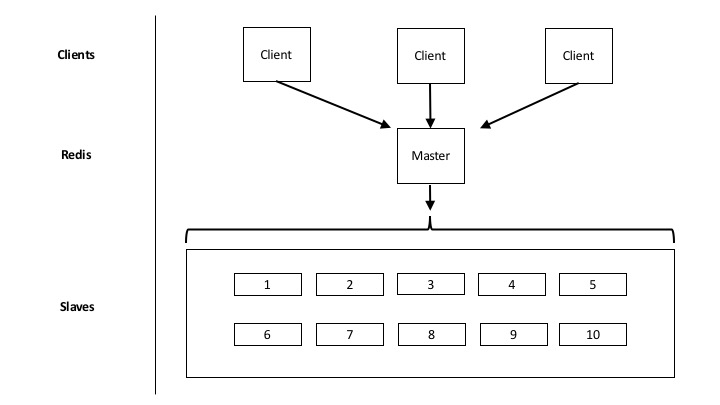
\includegraphics[width=6.5cm]{res/server_diagram.jpg}\\\indent
The above figure shows the design infrastructure. Clients send file system requests through the master server, which stores all metadata associated with the files and slave servers. Requests are accepted by a Java Spark web API through HTTP requests. On initial write, the master randomly chooses among the known slaves to store the file. This server is designated as the "original" server, and the file can never be removed from this server via rebalancing procedures. The original server is kept as a simple guarantee that a file will always exist somewhere in the file system. Redis, an open-source and networked server was chosen as the system to store metadata on master for two main reasons:
\begin{enumerate}
	\item In-memory: Many of the rebalancing procedures and metadata maintenance require accesses to a large portion of metadata. By keeping this in-memory, overhead for maintaining master is minimized. In-memory procedures done in master should be overshadowed by the actual I/O to slaves, which are known to take much longer to finish. 
	\item Data structure store: Redis supports storage of much more than just key-value pairs. This simplified our development process, as we could use its built-in set, map, and list operations. 
\end{enumerate}
In addition to a mapping of each file to its original server, the master server also maintains a mapping of each file to all duplicates, a mapping of each server to all files stored on that server, timestamps per file, and a buffer of the most recent files and servers accessed. Our implementation sets the buffer size at 40 for testing, but in production this can be much higher. DDDFS was primarily built with speed (reads) in mind and does not plan for many file modifications (simpler to instead create a new file). Thus, older unread file metadata can be un-cached from Redis memory and eventually garbage-collected (or backed up to disk).

\subsection*{Load Balancing Design}
We have conceived two operations for the DDDFS: file balancing and server balancing. For file balancing, the basic idea is to predict when a file will be read by many clients and to duplicate that file across many servers prior to that event. By doing so, clients can read in parallel, eliminating constraints imposed by network throughput or server performance. Server balancing focuses on a related idea when files on a specific server will be read by many clients. In this case, files are moved from the busy server to less busy servers. This should lead to the same performance improvements as file balancing. \\\indent
It is necessary for DDDFS to keep track of recent reads by clients in its metadata in order to perform these two operations.  The file balancing operation determines the number of desired replicas for each file using the recent read metadata, and duplicates or deletes files accordingly. Servers designated to store duplicates are chosen at random among the cluster. In the simplest algorithm, a file's desired number of replicas is proportional to the number of recent reads. In our implementation, file balancing occurs every 10 seconds and server balancing occurs every 22 seconds. These intervals can be modified to fit the specific needs and read requests of each application. Thus, DDDFS has only eventual consistency, depending on both the balancing operations and when each slave schedules its actual file transactions. Such a model is fitting for a system with a large number of reads of unlinked data. By implementing these two operations with low performance and space overhead, we hope to show that performance load balancing should be a consideration for future distributed file systems. 

Like HDFS, all metadata will be stored in memory on the central server, while the application data is separately stored on child nodes. Additionally, we will model our file movements and replications after HDFS not only for simplicity, but also as proof that such movements and replications can be done quickly (as shown by HDFS). By showing the viability of the low overhead "performance load balancer" in DDDFS, we aim to elucidate the possibility of using such a load balancer in existing file systems such as HDFS.

\section{Difficulties}
Difficulties were encountered for performance measurement as there was no easy way of simulating a large number of clients in a short period of time. Java Spark does not handle concurrent HTTP requests well so certain requests are never received. A more durable and mature framework such as Java Spring could provide guarantees on receiving requests. 

A difficulty encountered while using Redis was to find a memory and time-efficient algorithm for calculating how many duplicates were desired for a file. A naive algorithm would be to just keep access counts for every file from the creation of the file but that potentially uses memory exceeding the system (practical limit of around 100 GB).

The original plan centered around providing detailed diagnostic information to the file system and to the client, but our implementation provides no such information to the client. Instead, all of the information is used for file and server rebalancing. While this removes a level of control and significantly increases software complexity (especially for optimization algorithms), the client no longer has to analyze data in order to better schedule his own tasks, and can instead just send requests to the server and depend on the server to deliver good performance.

%------------------------------------------------

\section{Results}
Our implementation's source code can be found at \href{https://github.com/alexdao/LBDS}{https://github.com/alexdao/LBDS}. To demonstrate the functionality of DDDFS, a test suite is provided to simulate write (create) and read requests for many (large test) and a few (small test) transactions. File modifications are currently not supported. \\\indent
The large test begins with writing three files to DDDFS. These are written to three slave servers in the cluster chosen at random. We tested with a buffer size of 40 for past reads and a cluster size of 10 for the slaves.
\begin{verbatim}
File locations: 
file2: 8 
file3: 3 
file1: 8 
\end{verbatim}
After 8 read requests for file2, the read rebalancing operation kicks in and the results are as shown:
\begin{verbatim}
File locations: 
file2: 0 4 5 6 8 9 
file3: 0 8 
file1: 2 8 
\end{verbatim}
file2 had been duplicated on 5 more servers, in addition to singular duplications for file1 and file3 (files are guaranteed to be on at least 1 server). Next, 40 reads were performed for file3:
\begin{verbatim}
File locations: 
file2: 0 4 5 6 8 9 
file3: 0 1 2 3 4 5 6 7 8 9 
file1: 2 8 
\end{verbatim}
After so many read requests, file3 had been rebalanced and duplicated on all 10 servers in the cluster. Finally, 40 more reads were performed for file2 leading to these server states:
\begin{verbatim}
File locations: 
file2: 0 1 2 3 4 5 6 7 8 9 
file3: 0 2 3 
file1: 8 
\end{verbatim}
Since file2 was more heavily requested, it was duplicated across every server. In addition, requests for file3 had dropped off, and as such, the number of duplicates on servers decreased as well. These deletions are important to maximize space on servers and allow for future rebalancing to service heavy traffic of other files.
%------------------------------------------------

\section{Limitations}
A limitation of DDDFS is its inability to store relations between files as the entire file system is essentially a hash table. This means that traditional relations such as folders are lost within DDDFS. DDDFS filenames can be structured intelligently (with the filename essentially being a path), but this results in additional complexity and lost performance. 

Another limitation of the DDDFS is that there is currently no action verification in place. Requests processed by master possibly result in slave server actions, such as file movement. These actions are assumed to be received and processed by the slave servers. To overcome this limitation, two-phrase commit can be utilized, though for many small files, this may result in network and performance degradation.

\section{Future Work}

Performance load balancing is a resource optimization technique with large potential that the DDDFS only begins to explore. If the metadata overhead is kept small enough, there are many unexplored ways to further improve performance. Furthermore, we need more concrete evidence of the potential for performance improvement using performance load balancing.

\subsection*{Workload Analysis}
The GFS paper claims that the disproportionate access of a single file occurred in some rare cases, but that this was not a concern [2]. By benchmarking performance of existing distributed file systems and comparing the performance difference between a "regular" workload, a workload consisting of evenly distributed file accesses, and a workload with concentrated file accesses, we can see how much of a bottleneck concentrated file accesses can cause.

\subsection*{Rebalancing Algorithm}
The rebalancing algorithms implemented for the DDDFS are extremely simple. It is possible to use different algorithms, or improve upon the existing ones so inefficient changes do not occur. For example, moving a file $x$ from server 1 to server 2, then replicating file $x$ on server 1 would be inefficient. More work should be spent on avoiding such cases. An example of a completely different algorithm would be using heuristics to predict future accesses and the number of desired replicas. Currently, in server rebalancing, we move a random file from the most busy server to the least busy. Instead of a randomly chosen file, we could move the most heavily accessed files (in near $O(1)$ find speed). In addition, read balancing and server balancing are currently both performed at fixed intervals. The balancing should ideally be performed during lulls of activity. As the actual balancing process across slave servers is expensive (due to I/O), balance detection and calculation should be performed often but only executed when deemed necessary. 

\subsection*{Integration with HDFS}
Since DDDFS was designed with the workload of HDFS in mind, it would be interesting to observe the operation of a version of HDFS that uses performance load balancing. By benchmarking such a system, it would be possible to observe the performance overhead (though we have already deduced that it should be low) as well as the performance benefits, if there are any. Furthermore, we would be able to see if the DDDFS file balancing is fast enough to be performed in low activity periods. Such a system would be the most compelling argument for the efficacy of performance load balancing.	

Furthermore, DDDFS only performs operations on metadata for file accesses, server locations, and server data. Any distributed file system that provides an interface for accessing and controlling where files are stored in a cluster can be easily integrated with DDDFS as a layer on top to optimize performance. 

\subsection*{Combining Performance and Storage LB}
The ideal distributed file system would load balance so that there is a proportional amount of data and accesses on each server. While this may not always be possible, there should be algorithmic methods to get as close as possible. Finding an efficient way to do so would be a step towards creating an ideal DFS. 

%----------------------------------------------------------------------------------------
%	REFERENCE LIST
%----------------------------------------------------------------------------------------
\begin{thebibliography}{99} % Bibliography - this is intentionally simple in this template
\bibitem{Dynamic Load Balancing} Valeria Cardellini, Michele Colajanni, Philip S. Yu
\newblock Dynamic Load Balancing on Web-server Systems
\newblock \textit{1999 Internet Computing vol. 3, no. 3, pp. 28-39, May-June 1999}
\newblock IEEE. 1999.

\bibitem{GFS} Sanjay Ghemawat, Howard Gobioff, and Shun-Tak Leung
\newblock The Google File System
\newblock \textit{ACM Symposium on Operating Systems Principles}
\newblock Google. 19 October 2003.

\bibitem{Spark} Java-Spark
\newblock http://sparkjava.com/documentation.html

\bibitem{HDFS} Jeffrey J. Hanson
\newblock An introduction to the Hadoop Distributed File System
\newblock \textit{developerWorks}
\newblock IBM. 1 February 2011. 

\bibitem{Hadoop} Konstantin Shvachko, Hairong Kuang, Sanjay Radia, Robert Chansler
\newblock The Hadoop Distributed File System
\newblock \textit{MSST '10 Proceedings of the 2010 IEEE 26th Symposium on Mass Storage Systems and Technologies}
\newblock Yahoo!. 2010.

\bibitem{Redis} Redis
\newblock http://redis.io/

\end{thebibliography}


%----------------------------------------------------------------------------------------

\end{multicols}

\end{document}
